\chapter{ARM与嵌入式}

ARM Cortex主要有9种运行模式,每一种运行模式的代码及说明如下图\nameref{fig:arm_arch}所示
\begin{figure}[H]
  \centering
  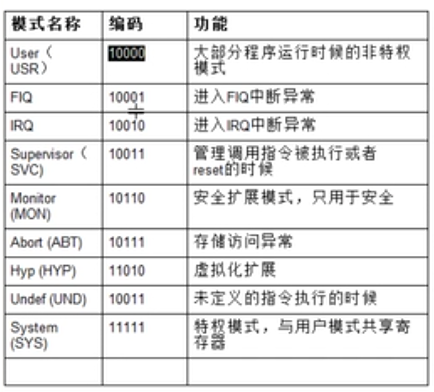
\includegraphics[scale=0.8]{arm_models.png}
  \caption{ARM的运行模式}
  \label{fig:arm_arch}
\end{figure}

ARM还拥有18个寄存器,每个寄存器长度为32位,R0~R12为通用寄存器,R13为栈指针寄存器(SP),R14为
链接指针寄存器(LP),R15为程序计数器(PC),如下图\nameref{fig:arm_reg}所示
\begin{figure}[H]
  \centering
  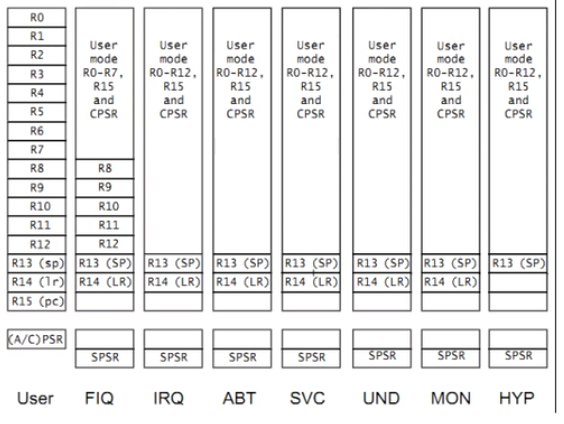
\includegraphics[scale=0.6]{arm_reg.png}
  \caption{ARM寄存器分类}
  \label{fig:arm_reg}
\end{figure}

除了这16个寄存器之外,ARM根据模式的不同,还有APSR(应用程序寄存器)/CPSR(当前程序寄存器)和SPSR(已存储程序寄存器)。
R0-R12寄存器,在所有模式(除快速中断模式)当中共享;快速中断(通常与硬件相关,FIQ)独占R8~R12寄存器;PC和CPSR寄存器是所有模式共享;
其余的寄存器基本是每种模式自己独占;用户模式(Usr)下不存在SPSR。

每一条ARM指令都是32位长度的,CPSR指令的格式大致如下图\nameref{fig:arm_command}所示:
\begin{figure}[H]
  \centering
  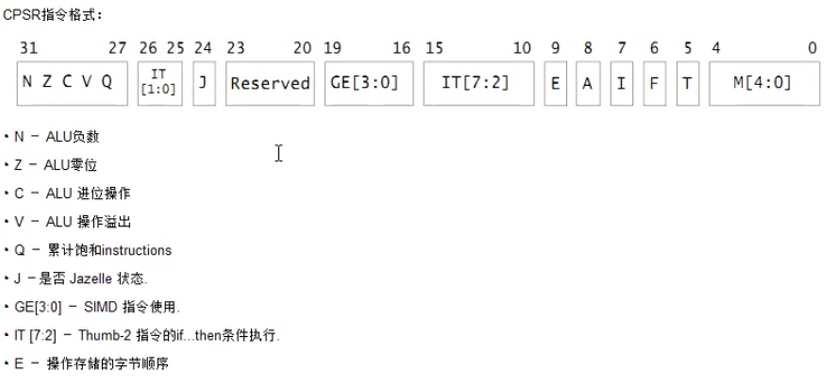
\includegraphics[width=\linewidth]{arm_command.png}
  \caption{ARM指令}
  \label{fig:arm_command}
\end{figure}

其中,指令的最后5位(M[4:0])正好表示本条指令的运行模式;第5位T,表示该指令是否使用是
Thumb指令集,1表示使用;第6位F表示FIQ,表示是否禁用FIQ中断;第7位I表示是否禁用IRQ;
第8位A表示是否禁用异步的abort;第9位E表示操作的字节序,即大小端;10-15位(IT[7:2])表示
Thumb2指令集当中的if-then条件执行;16-19位(GE[3:0])表示SIMD指令(单指令多数据);20-23位
为保留位;24位J表示Jazell状态,是否启用java加速;25-26(IT[1:0])表示Thumb指令集当中的if-then;
27到31分别为Q(累计饱和),V(ALU操作溢出),C(ALU进位操作),Z(ALU零位),N(ALU负数)。


